\begin{figure}[htbp]
			\centering
			\begin{tikzpicture}[
				scale=0.95,
				>=latex,
				trave/.style={line width=2pt},
				diagN/.style={black, line width=0.8pt},
				diagT/.style={black, line width=0.8pt},
				diagM/.style={black, line width=0.8pt},
				fibre/.style={dashed, gray!40, line width=0.6pt},
				]
				
				]
				
				% ── Parametri e macro dei vincoli (convenzione C06/C07) ──
				\def\tw{0.15}\def\thR{0.28}\def\rn{0.06}
				\def\rw{0.05}\def\bw{0.09}\def\gw{0.22}\def\hh{0.10}
				\def\vincoli{%
					% Cerniera in A=(0,0)
					\draw[thick] (0,0) -- (-\tw,-\thR) -- (\tw,-\thR) -- cycle;
					\draw[thick] (-\gw,-\thR) -- (\gw,-\thR);
					\foreach \x in {-0.16,-0.08,0,0.08,0.16}
					\draw[thin] (\x,-\thR) -- ++(-0.07,-\hh);
					% Carrello verticale in B=(3,3)
					\draw[thick] (3,3) -- (3-\tw,3-\thR) -- (3+\tw,3-\thR) -- cycle;
					\draw[thick] (3-\bw,3-\thR-\rw-0.01) circle (\rw);
					\draw[thick] (3+\bw,3-\thR-\rw-0.01) circle (\rw);
					\draw[thick] (3-\gw,3-\thR-2*\rw-0.04) -- (3+\gw,3-\thR-2*\rw-0.04);
					\foreach \x in {-0.16,-0.08,0,0.08,0.16}
					\draw[thin] (3+\x,3-\thR-2*\rw-0.04) -- ++(-0.07,-\hh);
					% Anellini (perni)
					\draw[thick, fill=white] (0,0) circle (\rn);
					\draw[thick, fill=white] (3,3) circle (\rn);
					% Etichette
					\node[left,  font=\small] at (-0.05, 0.12) {$A$};
					\node[right, font=\small] at ( 3.05, 3.08) {$B$};}
				
				% =========================================================
				% PANNELLO (a): N
				% =========================================================
				\begin{scope}[xshift=0cm]
					
					\draw[fibre] (0.0849,-0.0849) -- (3.0849,2.9151);
					\draw[trave] (0,0) -- (3,3);
					
					\vincoli
					
					\draw[diagN, line width=0.8pt]
					(0.6364,-0.6364) -- (0.8091,-0.2091) --
					(0.9818, 0.2182) -- (1.1546, 0.6454) --
					(1.3273, 1.0727) -- (1.5000, 1.5000) --
					(1.6727, 1.9273) -- (1.8454, 2.3546) --
					(2.0182, 2.7818) -- (2.1909, 3.2091) --
					(2.3636, 3.6364);
					
					\draw[diagN, line width=0.6pt]	(0,0) -- (0.6364,-0.6364);
					\draw[diagN, line width=0.6pt]	(3,3) -- (2.3636,3.6364);
					
					% Campiture N — P(t)=(3t,3t), tutti corretti
					% Prima metà f=(1-2t)*0.6364, t=0.05..0.45
					\draw[diagN,line width=0.3pt](0.15, 0.15)--(0.15+0.5728, 0.15-0.5728);
					\draw[diagN,line width=0.3pt](0.30, 0.30)--(0.30+0.5092, 0.30-0.5092);
					\draw[diagN,line width=0.3pt](0.45, 0.45)--(0.45+0.4456, 0.45-0.4456);
					\draw[diagN,line width=0.3pt](0.60, 0.60)--(0.60+0.3818, 0.60-0.3818);
					\draw[diagN,line width=0.3pt](0.75, 0.75)--(0.75+0.3182, 0.75-0.3182);
					\draw[diagN,line width=0.3pt](0.90, 0.90)--(0.90+0.2546, 0.90-0.2546);
					\draw[diagN,line width=0.3pt](1.05, 1.05)--(1.05+0.1910, 1.05-0.1910);
					\draw[diagN,line width=0.3pt](1.20, 1.20)--(1.20+0.1273, 1.20-0.1273);
					\draw[diagN,line width=0.3pt](1.35, 1.35)--(1.35+0.0637, 1.35-0.0637);
					% Seconda metà f=(2t-1)*0.6364, t=0.55..0.95
					\draw[diagN,line width=0.3pt](1.65, 1.65)--(1.65-0.0637, 1.65+0.0637);
					\draw[diagN,line width=0.3pt](1.80, 1.80)--(1.80-0.1273, 1.80+0.1273);
					\draw[diagN,line width=0.3pt](1.95, 1.95)--(1.95-0.1910, 1.95+0.1910);
					\draw[diagN,line width=0.3pt](2.10, 2.10)--(2.10-0.2546, 2.10+0.2546);
					\draw[diagN,line width=0.3pt](2.25, 2.25)--(2.25-0.3182, 2.25+0.3182);
					\draw[diagN,line width=0.3pt](2.40, 2.40)--(2.40-0.3818, 2.40+0.3818);
					\draw[diagN,line width=0.3pt](2.55, 2.55)--(2.55-0.4456, 2.55+0.4456);
					\draw[diagN,line width=0.3pt](2.70, 2.70)--(2.70-0.5092, 2.70+0.5092);
					\draw[diagN,line width=0.3pt](2.85, 2.85)--(2.85-0.5728, 2.85+0.5728);
					
					% N(A)<0 -> ominus vicino A; N(B)>0 -> oplus vicino B
					\node[diagN, font=\small] at (0.58,0.12) {$\boldsymbol{\ominus}$};
					\node[diagN, font=\small] at (2.45,2.9)	{$\boldsymbol{\oplus}$};
					
					
					\node[diagN, font=\scriptsize] at (0.20,-0.85)	{$\tfrac{\tilde{p}_0L\sqrt{2}}{4}$};
					\node[diagN, font=\scriptsize] at (2.10,3.85)	{$\tfrac{\tilde{p}_0L\sqrt{2}}{4}$};
					
					\node[font=\small] at (1.5,-0.80) {(a)};
					
				\end{scope}
				
				% =========================================================
				% PANNELLO (b): T — campiture identiche a N, segni invertiti
				% =========================================================
				\begin{scope}[xshift=4.0cm]
					
					\draw[fibre] (0.0849,-0.0849) -- (3.0849,2.9151);
					\draw[trave] (0,0) -- (3,3);
					
					\vincoli
					
					
					\draw[diagT, line width=0.8pt]
					(0.6364,-0.6364) -- (0.8091,-0.2091) --
					(0.9818, 0.2182) -- (1.1546, 0.6454) --
					(1.3273, 1.0727) -- (1.5000, 1.5000) --
					(1.6727, 1.9273) -- (1.8454, 2.3546) --
					(2.0182, 2.7818) -- (2.1909, 3.2091) --
					(2.3636, 3.6364);
					
					\draw[diagT, line width=0.6pt]
					(0,0) -- (0.6364,-0.6364);
					\draw[diagT, line width=0.6pt]
					(3,3) -- (2.3636,3.6364);
					
					% Campiture T — identiche a N
					\draw[diagT,line width=0.3pt](0.15, 0.15)--(0.15+0.5728, 0.15-0.5728);
					\draw[diagT,line width=0.3pt](0.30, 0.30)--(0.30+0.5092, 0.30-0.5092);
					\draw[diagT,line width=0.3pt](0.45, 0.45)--(0.45+0.4456, 0.45-0.4456);
					\draw[diagT,line width=0.3pt](0.60, 0.60)--(0.60+0.3818, 0.60-0.3818);
					\draw[diagT,line width=0.3pt](0.75, 0.75)--(0.75+0.3182, 0.75-0.3182);
					\draw[diagT,line width=0.3pt](0.90, 0.90)--(0.90+0.2546, 0.90-0.2546);
					\draw[diagT,line width=0.3pt](1.05, 1.05)--(1.05+0.1910, 1.05-0.1910);
					\draw[diagT,line width=0.3pt](1.20, 1.20)--(1.20+0.1273, 1.20-0.1273);
					\draw[diagT,line width=0.3pt](1.35, 1.35)--(1.35+0.0637, 1.35-0.0637);
					% Seconda metà f=(2t-1)*0.6364, t=0.55..0.95
					\draw[diagT,line width=0.3pt](1.65, 1.65)--(1.65-0.0637, 1.65+0.0637);
					\draw[diagT,line width=0.3pt](1.80, 1.80)--(1.80-0.1273, 1.80+0.1273);
					\draw[diagT,line width=0.3pt](1.95, 1.95)--(1.95-0.1910, 1.95+0.1910);
					\draw[diagT,line width=0.3pt](2.10, 2.10)--(2.10-0.2546, 2.10+0.2546);
					\draw[diagT,line width=0.3pt](2.25, 2.25)--(2.25-0.3182, 2.25+0.3182);
					\draw[diagT,line width=0.3pt](2.40, 2.40)--(2.40-0.3818, 2.40+0.3818);
					\draw[diagT,line width=0.3pt](2.55, 2.55)--(2.55-0.4456, 2.55+0.4456);
					\draw[diagT,line width=0.3pt](2.70, 2.70)--(2.70-0.5092, 2.70+0.5092);
					\draw[diagT,line width=0.3pt](2.85, 2.85)--(2.85-0.5728, 2.85+0.5728);
					
					% T(A)>0 -> oplus vicino A; T(B)<0 -> ominus vicino B
					\node[diagT, font=\small] at (0.58,0.12) {$\boldsymbol{\oplus}$};
					\node[diagT, font=\small] at (2.45,2.9)	{$\boldsymbol{\ominus}$};
					
					%\node[teal!60!black, font=\small] at (-0.55,1.50) {$T$};
					
					\node[diagT, font=\scriptsize] at (0.20,-0.85)	{$\tfrac{\tilde{p}_0L\sqrt{2}}{4}$};
					\node[diagT, font=\scriptsize] at (2.10,3.85)	{$\tfrac{\tilde{p}_0L\sqrt{2}}{4}$};
					
					\node[font=\small] at (1.5,-0.80) {(b)};
					
				\end{scope}
				
				% =========================================================
				% PANNELLO (c): M
				% =========================================================
				\begin{scope}[xshift=8.0cm]
					
					% Trave prima, poi fibre, poi diagramma M
					\draw[trave] (0,0) -- (3,3);
					\draw[fibre] (0.0849,-0.0849) -- (3.0849,2.9151);
					
					\vincoli
					
					
					% Diagramma M — poi campiture — poi ridisegno trave sopra
					\draw[diagM, line width=0.8pt]
					(0.0000, 0.0000) --
					(0.5800, 0.0200) --
					(1.0978, 0.1022) --
					(1.5534, 0.2466) --
					(1.9467, 0.4533) --
					(2.2778, 0.7222) --
					(2.5467, 1.0533) --
					(2.7534, 1.4466) --
					(2.8978, 1.9022) --
					(2.9800, 2.4200) --
					(3.0000, 3.0000);
					
					\draw[diagM,line width=0.3pt](0.15,0.15)--(0.15+0.1478,0.15-0.1478);
					\draw[diagM,line width=0.3pt](0.30,0.30)--(0.30+0.2800,0.30-0.2800);
					\draw[diagM,line width=0.3pt](0.45,0.45)--(0.45+0.3974,0.45-0.3974);
					\draw[diagM,line width=0.3pt](0.60,0.60)--(0.60+0.4978,0.60-0.4978);
					\draw[diagM,line width=0.3pt](0.75,0.75)--(0.75+0.5834,0.75-0.5834);
					\draw[diagM,line width=0.3pt](0.90,0.90)--(0.90+0.6534,0.90-0.6534);
					\draw[diagM,line width=0.3pt](1.05,1.05)--(1.05+0.7078,1.05-0.7078);
					\draw[diagM,line width=0.3pt](1.20,1.20)--(1.20+0.7467,1.20-0.7467);
					\draw[diagM,line width=0.3pt](1.35,1.35)--(1.35+0.7700,1.35-0.7700);
					\draw[diagM,line width=0.3pt](1.50,1.50)--(1.50+0.7778,1.50-0.7778);
					\draw[diagM,line width=0.3pt](1.65,1.65)--(1.65+0.7700,1.65-0.7700);
					\draw[diagM,line width=0.3pt](1.80,1.80)--(1.80+0.7467,1.80-0.7467);
					\draw[diagM,line width=0.3pt](1.95,1.95)--(1.95+0.7078,1.95-0.7078);
					\draw[diagM,line width=0.3pt](2.10,2.10)--(2.10+0.6534,2.10-0.6534);
					\draw[diagM,line width=0.3pt](2.25,2.25)--(2.25+0.5834,2.25-0.5834);
					\draw[diagM,line width=0.3pt](2.40,2.40)--(2.40+0.4978,2.40-0.4978);
					\draw[diagM,line width=0.3pt](2.55,2.55)--(2.55+0.3974,2.55-0.3974);
					\draw[diagM,line width=0.3pt](2.70,2.70)--(2.70+0.2800,2.70-0.2800);
					\draw[diagM,line width=0.3pt](2.85,2.85)--(2.85+0.1478,2.85-0.1478);
					
					% Ridisegno trave sopra le campiture
					\draw[trave] (0,0) -- (3,3);
					
					%\node[orange!80!black, font=\small] at (3.40,1.50) {$M$};
					
					\draw[diagM, line width=0.4pt, dashed]
					(1.50,1.50) -- (2.2778,0.7222);
					\node[diagM, font=\scriptsize, right]
					at (2.30,0.70)
					{$\tfrac{\tilde{p}_0L^2}{8}$};
					
					\node[font=\small] at (1.5,-0.80) {(c)};
					
				\end{scope}
				
			\end{tikzpicture}
			\caption{Trave inclinata di $\pi/4$ con carico
				verticale uniforme $\tilde{p}(x) = \tilde{p}_0$:
				diagrammi di $N(z)$ (a), $T(z)$ (b)
				e $M(z)$ (c).}
			\label{fig:stat_misto_inclinata_NTM}
		\end{figure}
